\subsection{Arduino}
{\tiny Written by: Felix}

\subsection{Arduino Implementation}

This document presents a comprehensive overview of the Arduino implementation, encompassing essential setup instructions, required libraries, a detailed flow chart elucidating the use case, a comprehensive sensor overview, and a schematic representation using Fritzing. Through this structured presentation, readers will gain a robust understanding of the technical components and operational procedures integral to this Arduino-based project.

\subsubsection{Arduino Setup}

The Arduino \textbf{Arduino Uno WiFi REV2} \cite{arduino_uno_wifi_rev2} component of the locker system project is developed using Arduino IDE version 2.3.2 \cite{arduino-software}. This development environment ensures a streamlined workflow, particularly when the Arduino is connected via USB, with logs displayed within the IDE's Terminal.

To set up the Arduino for this project, follow these steps:

\begin{enumerate}
    \item \textbf{Cloning the Arduino Repository}:
    Begin by cloning the Arduino repository referenced in the project documentation \cite{inventory-database-arduino}.
    
    \item \textbf{Wiring the Cables}:
    Refer to the Fritzing diagram provided in Section \ref{sec:ArduinoFritzing} Figure \ref*{fig:ardFritzing} to correctly wire the components for the Arduino setup.
    
    \item \textbf{Downloading Required Libraries}:
    Utilize the Arduino IDE specified in Section \ref{sec:ArduinoLibaries} to download and integrate the necessary libraries into your project.
    
    \item \textbf{Configuring WiFi Connection}:
    Update the WiFi credentials within the Arduino sketch as illustrated below:
    
    \begin{lstlisting}[language=C++, caption={WiFi Configuration in Arduino Sketch}]
    // WiFi Configuration
    #include <WiFiNINA.h>
    char ssid[] = "YOUR_SSID";
    char wifi_password[] = "YOUR_PASSWORD";
    \end{lstlisting}
    
    Replace \texttt{YOUR\_SSID} and \texttt{YOUR\_PASSWORD} with your WiFi network name (SSID) and password.
    
    \item \textbf{Creating a ThingSpeak Channel for Data Monitoring}:
    To monitor the wattage data from the sensors, you need to create a ThingSpeak channel online. This channel will serve as a platform to collect and visualize the sensor data in real-time. Obtain the Channel ID and Write API Key for your ThingSpeak channel.
    
    Include the following code snippet in your Arduino sketch to interface with ThingSpeak:
    
    \begin{lstlisting}[language=C++, caption={ThingSpeak Configuration in Arduino Sketch}]
    // ThingSpeak Configuration
    #include "ThingSpeak.h"
    unsigned long smart_room_channel_number = YOUR_CHANNEL_NUMBER;  // ThingSpeak Channel Number
    const char* write_API_KEY = "YOUR_WRITE_API_KEY";     // ThingSpeak Write API Key
    \end{lstlisting}
    
    Replace \texttt{smart\_room\_channel\_number} and \texttt{write\_API\_KEY} with your specific ThingSpeak channel number and Write API Key.

    \item \textbf{Setting up your Voltage}:
    Ensuring the correct voltage configuration is essential for accurate wattage measurements, as it directly impacts the output of electrical equations.

    To determine the appropriate voltage settings for your 
    Arduino project, consult international 
    standards or local electrical regulations 
    to identify the correct voltage rating for 
    your power grid, which can be found here \cite{rei-world-electricity-guide}

    \begin{lstlisting}[language=C++, caption={Setting Voltage in Arduino Sketch}]
    // Setting up Voltage for Power Grid
    int voltage = 220; // Default Voltage for Power Grid (in volts)
    \end{lstlisting}

    In the provided Arduino sketch code snippet, the `voltage` variable is initialized with a default value of 220 volts, which is commonly used in many regions. Modify this value according to the specific voltage rating of your local power grid to ensure accurate readings and safe operation of your voltage monitoring system.

\end{enumerate}

After setting up the development environment and configuring the Arduino,
proceed with starting the Arduino.
The LCD display will provide real-time status updates or prompts,
such as commands to close the door. 
The Arduino initializes in a consistent state upon startup.

Ensure adherence to this structured approach to establish a reliable 
and functional Arduino setup for the locker system project.

\subsubsection{List of Important Libraries and Versions}\label{sec:ArduinoLibaries}

The following list includes the most important libraries used in the Arduino implementation along with their versions:

\begin{itemize}
    \item \textbf{Servo} by Michael Margolis, Arduino 1.2.1 (Servo Motor) \\ Controls the movement of servos for locking and unlocking the locker door.
    \item \textbf{Grove - LCD RGB Backlight} by Seeed Studio 1.0.0 (Display LCD) \\ Displays information and status messages on the locker system interface.
    \item \textbf{ArduinoJson} by Benoit Blanchon 7.0.4 \\ Parses and manipulates JSON data for communication and data exchange.
    \item \textbf{WifiNINA} by Arduino 1.8.14 \\ Enables Wi-Fi connectivity for accessing online services (FastAPI) and remote monitoring (ThingSpeak).
    \item \textbf{Keypad} by Mark Stanley, Alexander Brevig 3.1.1 (Keypad) \\ Allows user input for password authentication and interaction with the locker system.
    \item \textbf{ThingSpeak} by MathWorks 2.0.1 \\ Sends sensor data to ThingSpeak for real-time monitoring and visualization.
\end{itemize}
\newpage
\subsubsection{Flow Chart}
In this section, we provide a detailed flow chart illustrating the step-by-step process of utilizing our 
locker system for charging or renting items. The flow chart serves as a visual guide to clarify the 
functionality of our product, outlining the precise sequence of actions required to either charge your 
item securely within our lockers or efficiently rent an item from our locker device. 
This visual representation will enhance your understanding of how our innovative locker system operates,
ensuring a seamless and user-friendly experience for our customers. 
Let's delve into the flow chart to explore the intricacies of our product functionality.

\begin{figure}[h]
    \centering
    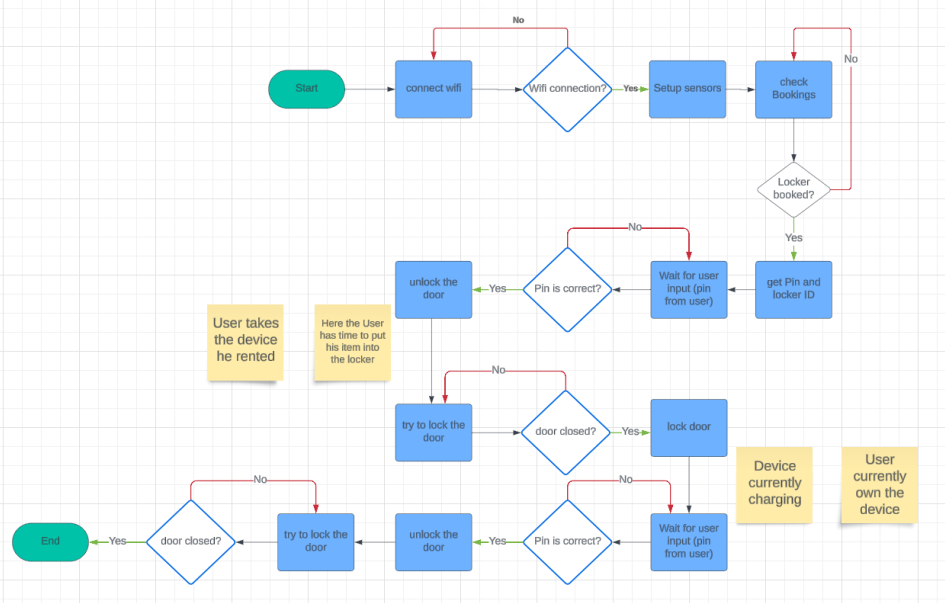
\includegraphics[width = \textwidth]{images/Arduino/flowchart_ard.png}
    \caption{Flow chart for charging and renting items}
    \label{fig:flowchart}
\end{figure}

\newpage

\subsubsection{Sensors Overview}\label{sec:ArduinoSensors}

\begin{enumerate}
    \item \textbf{Keypad}  
    
    \textbf{Reference}: Tutorial available at \cite{keypad-tutorial}
    
    \textbf{Purpose}: The keypad allows user input for controlling and interacting with the Arduino locker system. It enables entering the PIN code or commands like \# for starting to enter the password or \* for confirming the password, to operate the system securely.
    
    \textbf{Functionality}: The Arduino interprets the key presses from the keypad matrix and executes corresponding actions based on the input received.
    
    \begin{figure}[h]
        \centering
        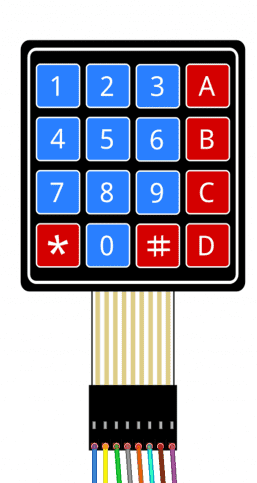
\includegraphics[width=0.4\textwidth]{images/Arduino/keypad_image.png} % Image placeholder
        \caption{Keypad}
    \end{figure}
\newpage

    \item \textbf{LCD-Screen}
    
    \textbf{Reference}: Details available at \cite{seeedstudio-lcd}
    
    \textbf{Purpose}: The LCD screen displays real-time information and system status to users, providing visual feedback about the locker system's operation.
    
    \textbf{Functionality}: The Arduino sends commands to the LCD screen to display text and graphics, enhancing user interaction and system monitoring capabilities.
    
    \begin{figure}[h]
        \centering
        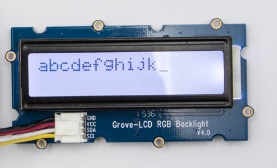
\includegraphics[width=0.5\textwidth]{images/Arduino/lcd_image.png} % Image placeholder
        \caption{LCD Screen}
    \end{figure}
\newpage
    \item \textbf{Current Sensor}
    
    \textbf{Reference}: Follow this \cite{current-sensor-tutorial} for implementation details
    
    \textbf{Purpose}: The current sensor measures electrical current flowing through a circuit, enabling monitoring of power consumption and detecting anomalies.
    
    \textbf{Functionality}: The Arduino reads analog voltage signals from the current sensor to calculate current values, which can be used for power management and safety monitoring.
    
    \begin{figure}[h]
        \centering
        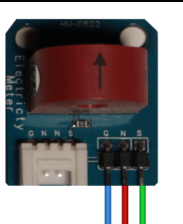
\includegraphics[width=0.4\textwidth]{images/Arduino/current_sensor_image.png} % Image placeholder
        \caption{Current Sensor}
    \end{figure}
\newpage
    \item \textbf{Door Sensor}
    
    \textbf{Reference}: Learn more about Arduino door sensors from this \cite{door-sensor-tutorial}
    
    \textbf{Purpose}: The door sensor detects the state (open or closed) of the locker door, providing security and triggering actions based on door status changes.
    
    \textbf{Functionality}: The Arduino reads digital signals from the door sensor to determine the door's position and reacts accordingly, such as activating the locking mechanism.
    
    \begin{figure}[h]
        \centering
        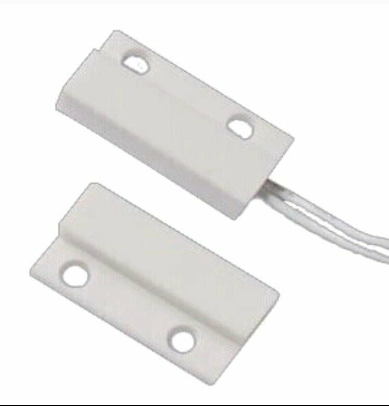
\includegraphics[width=0.5\textwidth]{images/Arduino/door_sensor_image.png} % Image placeholder
        \caption{Door Sensor}
    \end{figure}
    \newpage

    \item \textbf{Servo Motor}  
    
    \textbf{Reference}: Tutorial available at \cite{arduino-micro-servos}
    
    \textbf{Purpose}: The servo motor controls the mechanical movement of the locker's locking mechanism, enabling remote operation and automation.
    
    \textbf{Functionality}: The Arduino sends PWM signals to the servo motor to position it at specific angles, allowing precise control over the locking and unlocking of the locker.
    
    \begin{figure}[h]
        \centering
        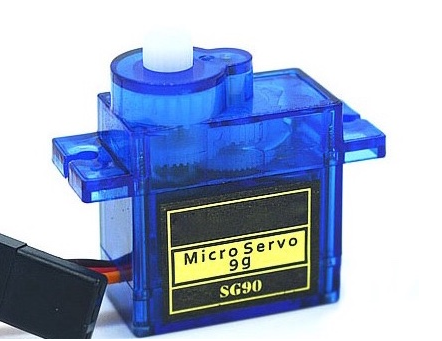
\includegraphics[width=0.5\textwidth]{images/Arduino/servo.png} % Image placeholder
        \caption{Servo Motor }
    \end{figure}
    
\end{enumerate}


\newpage
\subsubsection{Fritzing}\label{sec:ArduinoFritzing}
The image depicted in Figure \ref{fig:ardFritzing} illustrates the correct arrangement and connections of cables and components required for setting up the Arduino system as described in this guide. This visual guide, created using Fritzing software, provides a clear representation of how to wire the Arduino board with various sensors and peripherals. Referencing this diagram will ensure accurate implementation of the hardware setup outlined in the instructions.

\begin{figure}[h]
    \centering
    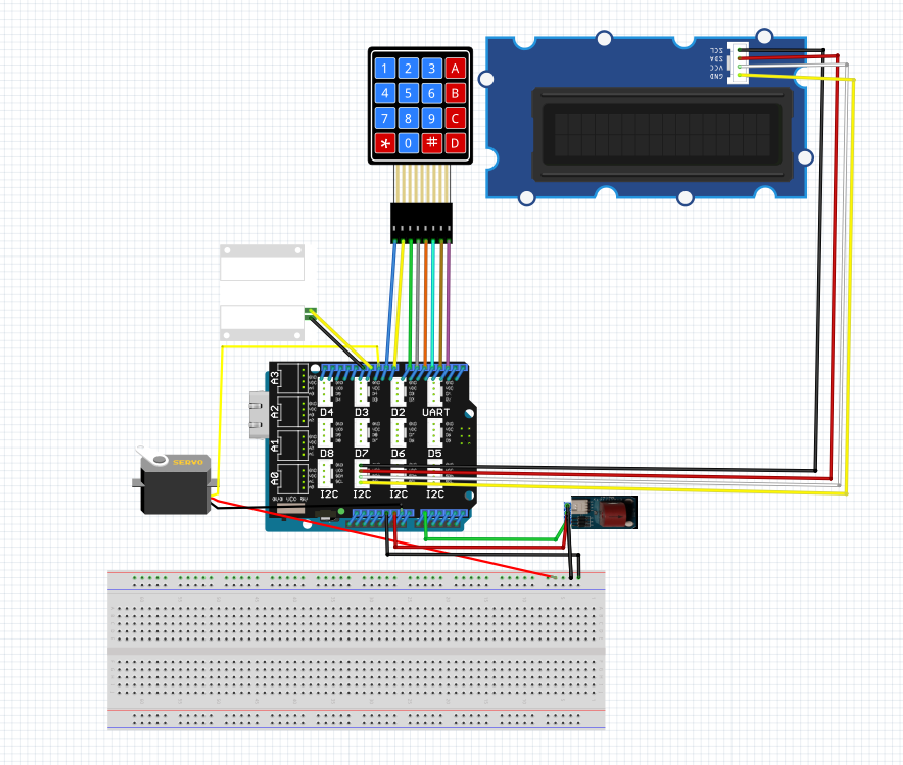
\includegraphics[width=0.8\textwidth]{images/Arduino/arduino_fritzing_curcuit.png}
    \caption{Arduino Fritzing setup}
    \label{fig:ardFritzing}
\end{figure}


